\documentclass[conference]{IEEEtran}
\IEEEoverridecommandlockouts
\usepackage{cite}
\usepackage{amsmath,amssymb,amsfonts}
\usepackage{booktabs}
\usepackage{enumitem}
\usepackage{tikz}
\usetikzlibrary{arrows.meta,positioning}

\newcommand{\sat}{\operatorname{sat}}
\newcommand{\diag}{\operatorname{diag}}

\begin{document}

\title{High-Definition Haptic Device:\\ Hardware Physics, Identification, Modelling, and the Complete Controller Suite\\
{\footnotesize Mathematical foundations for offline simulation, digital-twin, and hardware execution}}

\author{\IEEEauthorblockN{Gandhi Contreras}
\IEEEauthorblockA{\textit{Electrical and Computer Engineering}, New Mexico State University, Las Cruces, NM, USA \\ gandhico@nmsu.edu}}

\maketitle

\begin{abstract}
A haptic device is a robot whose ``task'' is the force felt by a human hand: it must be transparent when simulating free space and stiff when simulating contact, with stability guaranteed against the one element no designer controls --- the operator. This paper develops the mathematics of a high-definition pantograph-class haptic interface end to end: the direct-drive actuation chain built for torque fidelity (no gearbox, capstan or direct transmission), the linkage kinematics with Jacobian force mapping, the device dynamics in end-effector coordinates, identification of inertia, friction, and torque constants at the fidelity haptics demands, the rendering laws (impedance and admittance, the virtual wall), the passivity and virtual-coupling framework that governs stability of the sampled loop, and the controller suite --- PID, LQR, LQG, backstepping, sliding mode, and NMPC --- reinterpreted for force-domain objectives.
\end{abstract}

\begin{IEEEkeywords}
Haptics, impedance control, admittance control, passivity, virtual wall, transparency, Jacobian, backstepping, SMC, NMPC.
\end{IEEEkeywords}

%====================================================================
\section{Introduction}
Let $q\in\mathbb R^n$ be the joint angles of the linkage ($n = 2$ planar pantograph or $n=3$ with a third axis), $x = f(q)\in\mathbb R^n$ the end-effector (stylus/handle) position, and $J(q) = \partial f/\partial q$ the Jacobian. The device applies the hand force
\begin{equation}
F_h = J^{-\!\top}(q)\,\tau,
\label{eq:forcemap}
\end{equation}
so \emph{torque fidelity is force fidelity}: every parasitic torque (cogging, friction, inertia) is felt directly. This inverts the usual robotics priorities --- the hardware is designed so the \emph{model is small}, and control renders virtual dynamics rather than tracking trajectories.

%====================================================================
\section{Hardware Physics}

\begin{figure*}[!t]
\centering
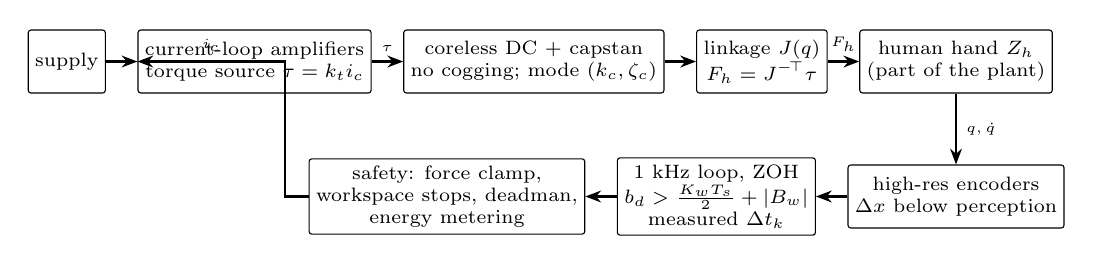
\begin{tikzpicture}[
  node distance=3mm and 4mm,
  blk/.style={draw, rounded corners=1pt, align=center, font=\scriptsize, inner sep=2.5pt, minimum height=8mm},
  lbl/.style={font=\tiny, align=center},
  arr/.style={-{Stealth[length=2mm]}, thick}
]

\node[blk] (sup) {supply};
\node[blk, right=of sup] (amp) {current-loop amplifiers\\ torque source $\tau = k_t i_c$};
\node[blk, right=of amp] (mot) {coreless DC + capstan\\ no cogging; mode $(k_c,\zeta_c)$};
\node[blk, right=of mot] (link) {linkage $J(q)$\\ $F_h = J^{-\!\top}\tau$};
\node[blk, right=of link] (hand) {human hand $Z_h$\\ (part of the plant)};
\node[blk, below=9mm of hand] (enc) {high-res encoders\\ $\Delta x$ below perception};
\node[blk, left=of enc] (loop) {1 kHz loop, ZOH\\ $b_d > \tfrac{K_wT_s}{2} + |B_w|$\\ measured $\Delta t_k$};
\node[blk, left=of loop] (safe) {safety: force clamp,\\ workspace stops, deadman,\\ energy metering};
\draw[arr] (sup) -- (amp);
\draw[arr] (amp) -- node[lbl, above] {$\tau$} (mot);
\draw[arr] (mot) -- (link);
\draw[arr] (link) -- node[lbl, above] {$F_h$} (hand);
\draw[arr] (hand) -- node[lbl, right] {$q,\dot q$} (enc);
\draw[arr] (enc) -- (loop);
\draw[arr] (loop) -- (safe);
\draw[arr] (safe.west) -- ++(-3mm,0) |- node[lbl, pos=0.75, above] {$i_c$} (amp.west);
\end{tikzpicture}
\caption{Haptic device signal chain: the human is inside the loop; the sampled-passivity bound ties renderable stiffness to loop rate and physical damping.}
\label{fig:chain}
\end{figure*}
\subsection{Actuation for transparency}
Brushed, coreless (ironless-rotor) DC motors in \emph{direct drive} or low-ratio capstan-cable transmission: no gearbox means no backlash and reflected friction/inertia scale with $N_g^2 = 1$; coreless rotors eliminate cogging torque (no iron teeth) and minimize rotor inertia. The electrical model is the standard $L_a\dot i + R_m i + k_e\dot q_m = v$, $\tau_m = k_t i$, but haptics closes a \emph{current} (torque) loop in the drive: with a high-bandwidth current controller the motor is a torque source $\tau_m = k_t\,i_c$ up to the amplifier's current and voltage compliance limits; back-EMF then appears to the mechanism only as the voltage-compliance ceiling $|\dot q|\le (V_{\max} - R_m i)/k_e$. Capstan transmissions (ratio $N_c$) multiply torque with rolling --- not sliding --- contact: negligible backlash, small elasticity $k_c$ that appears as a high-frequency transmission mode.

\subsection{Sensing and the loop}
High-line-count encoders on the motor shafts (haptic ``definition'' is resolution: position quantum $\Delta x \approx q_{\mathrm{enc}}\,\|J\|/N_c$ must be below human perceptual thresholds); velocities by filtered differentiation --- the dominant noise source in damping rendering. Loop rate is the defining constraint of the field: haptic rendering runs at $f_s \ge 1$~kHz because (Section~\ref{sec:passivity}) the renderable stiffness scales with $1/T_s$. Measured-$\Delta t$ discipline applies as on all our platforms. Safety: force/current clamps, workspace software stops inside the mechanical stops, velocity watchdog (runaway detection), deadman/handle-presence logic, and power-on state machine that ramps torque authority.

%====================================================================
\section{Modelling}
\subsection{Kinematics and statics}
For the five-bar pantograph with actuated proximal links $(q_1, q_2)$, link lengths $(l_1, l_2)$, base separation $d$: $x = f(q)$ by the standard two-circle intersection; $J(q)$ its Jacobian; singular configurations where $\det J = 0$ bound the usable workspace (force capability $\to$ anisotropic: the force ellipsoid $\{J^{-\!\top}\tau : \|\tau\|\le\bar\tau\}$ degenerates).

\subsection{Dynamics}
Euler--Lagrange in joint space,
\begin{equation}
M(q)\ddot q + C(q,\dot q)\dot q + F_v\dot q + \tau_c\tanh(\dot q/\epsilon) = \tau + J^{\!\top}(q)\,F_{\mathrm{hand}},
\label{eq:hapdyn}
\end{equation}
gravity absent (planar horizontal) or a small $G(q)$ otherwise; the hand force enters as an exogenous input --- the human is part of the plant. In end-effector coordinates, with $\Lambda = J^{-\!\top}MJ^{-1}$ the operational-space inertia,
\begin{equation}
\Lambda(q)\ddot x + \mu(q,\dot q)\dot x + J^{-\!\top}\!\bigl(F_v\dot q + \ldots\bigr) = F_a + F_{\mathrm{hand}},
\label{eq:opspace}
\end{equation}
$F_a = J^{-\!\top}\tau$ the actuation force. \emph{Transparency} is the requirement that the left side of \eqref{eq:opspace} be imperceptible: $\|\Lambda\|, $ friction, and vibration modes below perception thresholds in the target band (DC--40~Hz kinesthetic, up to $\sim$1~kHz cutaneous).

%====================================================================
\section{Identification}

\begin{figure}[!t]
\centering
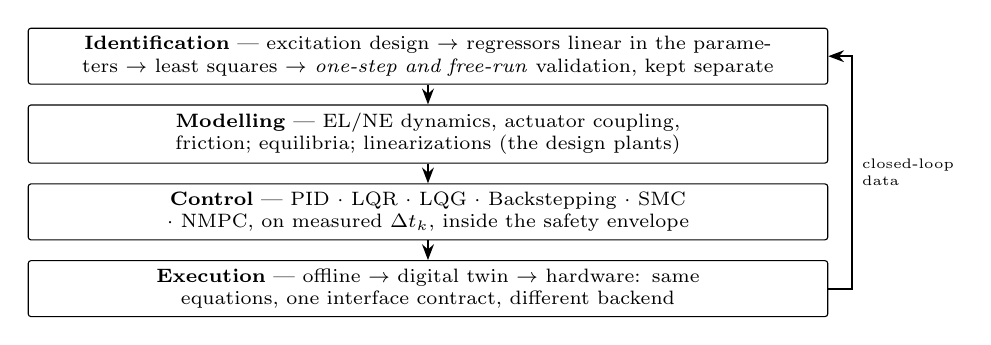
\begin{tikzpicture}[
  node distance=2.5mm,
  blk/.style={draw, rounded corners=1pt, align=center, font=\scriptsize, inner sep=3pt, text width=0.82\columnwidth},
  arr/.style={-{Stealth[length=2mm]}, thick}
]
\node[blk] (id) {\textbf{Identification} --- excitation design $\to$ regressors linear in the parameters $\to$ least squares $\to$ \emph{one-step and free-run} validation, kept separate};
\node[blk, below=of id] (mod) {\textbf{Modelling} --- EL/NE dynamics, actuator coupling, friction; equilibria; linearizations (the design plants)};
\node[blk, below=of mod] (ctl) {\textbf{Control} --- PID $\cdot$ LQR $\cdot$ LQG $\cdot$ Backstepping $\cdot$ SMC $\cdot$ NMPC, on measured $\Delta t_k$, inside the safety envelope};
\node[blk, below=of ctl] (exe) {\textbf{Execution} --- offline $\to$ digital twin $\to$ hardware: same equations, one interface contract, different backend};
\draw[arr] (id) -- (mod);
\draw[arr] (mod) -- (ctl);
\draw[arr] (ctl) -- (exe);
\draw[arr] (exe.east) -- ++(3mm,0) |- node[font=\tiny, pos=0.25, right, align=left] {closed-loop\\ data} (id.east);
\end{tikzpicture}
\caption{The workflow every platform in this series follows: identification feeds modelling, modelling feeds the controller suite, and all stages run unchanged across the three execution targets; closed-loop records return to identification.}
\label{fig:workflow}
\end{figure}
Haptic-grade identification targets the parasitics themselves. E1) \emph{torque constants} $k_t$ per axis by force-sensor calibration at the handle through \eqref{eq:forcemap} (static, multiple poses --- also validates $J$). E2) \emph{friction}: constant-velocity sweeps map $\tau_f(\dot q)$ directly (Stribeck curve); breakaway measured by torque ramps at rest. E3) \emph{inertia}: \eqref{eq:hapdyn} is linear in the link inertial parameters; chirp excitation with the handle free, regressor least squares; cross-check via the measured apparent mass at the handle ($\|F\|/\|\ddot x\|$ at mid-band). E4) \emph{transmission mode}: frequency response to torque excitation reveals the capstan resonance $(k_c, \zeta_c)$ that caps stable rendering gains. Validation: one-step and free-run on held-out records, plus the haptic-specific metric --- rendered-vs-commanded impedance error over the perception band.

%====================================================================
\section{Rendering Laws and Passivity}\label{sec:passivity}
\subsection{Impedance and admittance}
\emph{Impedance rendering} (native for this direct-drive class): measure motion, output force,
\begin{equation}
F_a = -K_v\,(x - x_w) - B_v\,\dot x \quad\text{(virtual spring--damper)},
\label{eq:impedance}
\end{equation}
with \eqref{eq:forcemap} mapping to torques. \emph{Admittance rendering} (for stiff, geared devices): measure force, servo motion through a position loop --- included for completeness; the duality is exact (impedance renders low impedances well, admittance high ones).

\subsection{The virtual wall and the sampled-data limit}
The canonical benchmark is the unilateral wall $F_a = -K_w x - B_w\dot x$ for $x > 0$, else $0$. Discretization with ZOH and one-sample delay injects energy; the classical passivity condition bounds the renderable stiffness:
\begin{equation}
\boxed{\; b_d \;>\; \frac{K_w T_s}{2} + |B_w| \;}
\label{eq:colgate}
\end{equation}
where $b_d$ is the device's \emph{physical} damping (Colgate--Schenkel): sampled stiffness must be backed by real dissipation. This inequality is the mathematical reason for the 1~kHz loop, for quantization-aware velocity filtering (quantization noise through $B_w$ also pumps energy), and for valuing intrinsic damping that transparency would otherwise want to remove --- the central design tension of haptics.

\subsection{Two-port framework}
Rendering a virtual environment $Z_e(s)$ to a human $Z_h(s)$ through the device and the discrete loop is a two-port network; unconditional stability for all passive $Z_h, Z_e$ is guaranteed if the port is passive,
$\int_0^t F^{\!\top}\dot x\,d\sigma \ge -E_0$, enforced constructively by a \emph{virtual coupling} (series spring--damper between device and environment) or at run time by a \emph{passivity observer/controller} that meters injected energy and dissipates the excess --- the modern generalization of \eqref{eq:colgate}.

%====================================================================
\section{Control Suite (force-domain objectives)}
\subsection{PID}
(i) In impedance form, \eqref{eq:impedance} \emph{is} PD in disguise --- gains are the rendered physics, bounded by \eqref{eq:colgate}. (ii) For admittance or calibration tasks, joint PID position loops with anti-windup; integral action is used sparingly (it destroys the passivity of the rendered port at low frequency).

\subsection{LQR / LQG}
On the linearized \eqref{eq:opspace} augmented with the transmission mode, LQR designs the damping/stiffness injection optimally against torque cost --- useful as \emph{optimal virtual coupling} synthesis; LQG adds the Kalman velocity estimate from quantized encoders (the principled replacement for ad hoc velocity filters), with the caveat that the estimator's phase lag re-enters the passivity budget \eqref{eq:colgate}.

\subsection{Backstepping}
For admittance-type tracking through the actuator dynamics: $z_1 = x - x_d$, virtual velocity $\dot x^d = \dot x_d - c_1 z_1$; $z_2 = \dot x - \dot x^d$; force from \eqref{eq:opspace}; a third stage pushes through the current loop when its bandwidth is not negligible. $V = \tfrac12(z_1^{\!\top}z_1 + z_2^{\!\top}\Lambda z_2)$, $\dot V = -\sum c_i\|z_i\|^2$ using the skew symmetry of $\dot\Lambda - 2\mu$.

\subsection{Sliding mode}
$s = \dot e + \lambda e$ on position (admittance) or on force error (impedance with force sensing); equivalent control from \eqref{eq:opspace}; switching gain sized to the \emph{measured} friction uncertainty from E2; boundary layer above the velocity-estimate noise floor --- chatter is uniquely unacceptable here because the human feels it directly (it is a tactile artifact, not just wear).

\subsection{NMPC}
Receding horizon on \eqref{eq:hapdyn} with the virtual environment as constraint set: minimize deviation from the desired rendered impedance subject to torque limits, workspace stops, and an explicit \emph{energy budget constraint} $\sum_k F_k^{\!\top}\dot x_k\,\Delta t \ge -E_{\mathrm{max}}$ --- predictive passivity enforcement, the formulation where NMPC offers something the classical laws cannot: constraint-aware transparency near the actuator limits. Millisecond horizons at 1~kHz demand the full set of real-time reductions validated on our other platforms.

%====================================================================
\section{Execution Modes and Conclusion}
Offline: \eqref{eq:hapdyn} against a human-arm impedance model $Z_h$ (mass--spring--damper ranges from the literature) with quantization/ZOH/delay injected --- the virtual wall limit \eqref{eq:colgate} is reproduced numerically before touching hardware. Digital twin: the rendered environment itself is software, so the twin is the natural development target. Hardware: the physical device under the safety envelope with energy-metered rendering. The complete mathematics --- torque-fidelity hardware physics, Jacobian force mapping, operational-space dynamics, parasitic-grade identification, the passivity-bounded rendering laws, and the six-controller suite in force-domain form --- define what ``high definition'' means quantitatively: resolution, rate, and dissipation budgets that close \eqref{eq:colgate} at stiffness levels worth feeling.

\bibliographystyle{IEEEtran}
\begin{thebibliography}{9}
\bibitem{colgate1997} J.~E. Colgate and G.~G. Schenkel, ``Passivity of a class of sampled-data systems: Application to haptic interfaces,'' \emph{J. Robot. Syst.}, vol.~14, no.~1, 1997.
\bibitem{hannaford2002} B.~Hannaford and J.-H. Ryu, ``Time-domain passivity control of haptic interfaces,'' \emph{IEEE Trans. Robot. Autom.}, vol.~18, no.~1, 2002.
\bibitem{hogan1985} N.~Hogan, ``Impedance control: An approach to manipulation,'' \emph{ASME J. Dyn. Syst. Meas. Control}, vol.~107, 1985.
\bibitem{siciliano2009} B.~Siciliano, L.~Sciavicco, L.~Villani, and G.~Oriolo, \emph{Robotics: Modelling, Planning and Control}. Springer, 2009.
\bibitem{khalil2002} H.~K. Khalil, \emph{Nonlinear Systems}, 3rd ed. Prentice Hall, 2002.
\bibitem{utkin1992} V.~Utkin, \emph{Sliding Modes in Control and Optimization}. Springer, 1992.
\bibitem{rawlings2017} J.~B. Rawlings, D.~Q. Mayne, and M.~Diehl, \emph{Model Predictive Control}, 2nd ed. Nob Hill, 2017.
\end{thebibliography}

\end{document}
